\documentclass[tikz]{standalone}
\usepackage{pgfplots}
\pgfplotsset{compat=newest}
\pgfplotsset{every axis legend/.append style={%
cells={anchor=west}}
}
\usetikzlibrary{arrows}
\tikzset{>=stealth'}
\usepgfplotslibrary{groupplots}
\begin{document}
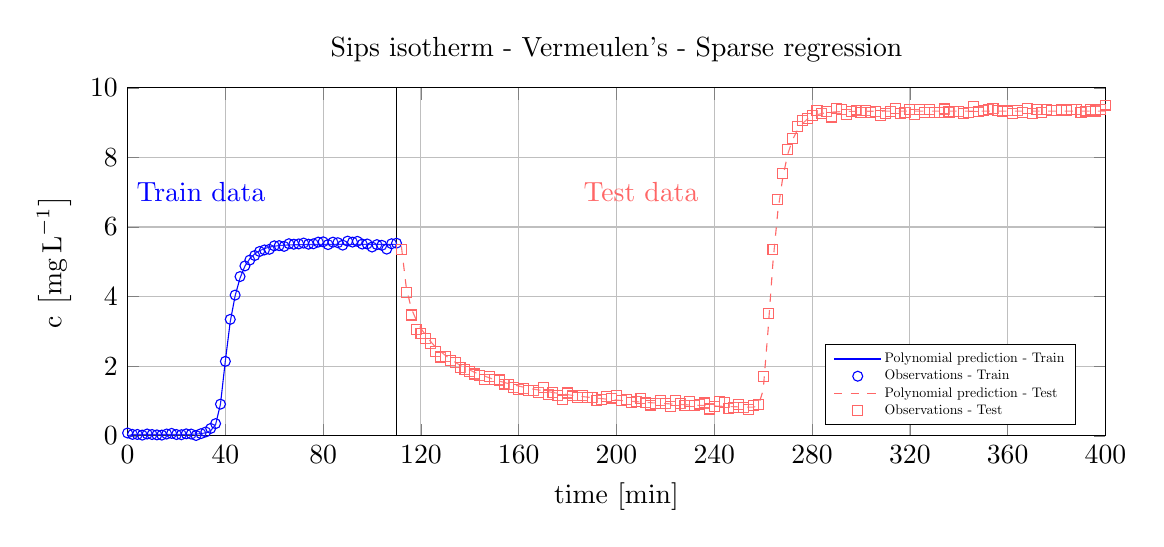
\begin{tikzpicture}[]
\begin{groupplot}[group style={horizontal sep = 2.75cm, vertical sep = 2.0cm, group size=1 by 1}]

\nextgroupplot [
  height = {6cm},
  legend pos = {south east},
  ylabel = {$\textrm{c}\,\left[\textrm{mg}\,\textrm{L}^{-1}\right]$},
  title = {Sips isotherm - Vermeulen's - Sparse regression},
  xmin = {0},
  xmax = {400},
  ymax = {10},
  xlabel = {time [min]},
  grid = both, ytick = {0, 2, 4, 6, 8, 10}, xtick = {0, 40, 80,...,400}, legend style={nodes={scale=0.5, transform shape}},
  ymin = {0},
  width = {14cm}
]

\addplot+[
  mark = {none},
  blue
] coordinates {
  (0.0, 0.001)
  (2.0, 0.03598034386859372)
  (4.0, 0.03598044005690836)
  (6.0, 0.03598106118312176)
  (8.0, 0.03598358719995875)
  (10.0, 0.03599171978125994)
  (12.0, 0.036013566980952545)
  (14.0, 0.03606440618823638)
  (16.0, 0.036176587269946235)
  (18.0, 0.036412097743190826)
  (20.0, 0.03687743941763035)
  (22.0, 0.03775814868713253)
  (24.0, 0.039461724879649863)
  (26.0, 0.042728057061778214)
  (28.0, 0.04892093001112)
  (30.0, 0.0610592781037642)
  (32.0, 0.08713303246459865)
  (34.0, 0.1489096814124854)
  (36.0, 0.32012512166329193)
  (38.0, 0.912982097417982)
  (40.0, 2.1615699732512317)
  (42.0, 3.2814759296473746)
  (44.0, 4.027208885664269)
  (46.0, 4.533936822306512)
  (48.0, 4.877382627156062)
  (50.0, 5.091647884887324)
  (52.0, 5.229214239322522)
  (54.0, 5.3202497411801115)
  (56.0, 5.381511420803591)
  (58.0, 5.423071709033203)
  (60.0, 5.44963238907842)
  (62.0, 5.466365069308465)
  (64.0, 5.477543386245632)
  (66.0, 5.485907374459232)
  (68.0, 5.490211578862804)
  (70.0, 5.493855486268875)
  (72.0, 5.495964400319243)
  (74.0, 5.49720431988632)
  (76.0, 5.49813707583184)
  (78.0, 5.498775063530214)
  (80.0, 5.499184136616296)
  (82.0, 5.499456913820979)
  (84.0, 5.499658348234681)
  (86.0, 5.499783221526464)
  (88.0, 5.499845779668417)
  (90.0, 5.499891414302534)
  (92.0, 5.49993478319171)
  (94.0, 5.499950508293548)
  (96.0, 5.499966378879785)
  (98.0, 5.499976379898237)
  (100.0, 5.49998216579163)
  (102.0, 5.499988475881686)
  (104.0, 5.499993274259817)
  (106.0, 5.499994832501939)
  (108.0, 5.499997785023199)
  (110.0, 5.499999380906137)
};
\addlegendentry{{}{Polynomial prediction - Train}}

\addplot+[
  only marks = {true},
  blue, mark = *, mark options={scale=0.9, fill=white, fill opacity = 0.1}
] coordinates {
  (0.0, 0.07979761550028977)
  (2.0, 0.03932261258896529)
  (4.0, 0.038201433546141174)
  (6.0, 0.019532051131636242)
  (8.0, 0.05162122358995544)
  (10.0, 0.036636979847575864)
  (12.0, 0.02610066095615494)
  (14.0, 0.020544541951698646)
  (16.0, 0.051078474010430044)
  (18.0, 0.06902369231383867)
  (20.0, 0.03609206992056761)
  (22.0, 0.03012861872274943)
  (24.0, 0.05610300247064698)
  (26.0, 0.049761318477107054)
  (28.0, 0.008436716584130144)
  (30.0, 0.06112199837561394)
  (32.0, 0.11015114775807987)
  (34.0, 0.2115545362710542)
  (36.0, 0.34965746059346714)
  (38.0, 0.909138051938194)
  (40.0, 2.1391022643980033)
  (42.0, 3.346683858310454)
  (44.0, 4.044166147615041)
  (46.0, 4.5763640797684255)
  (48.0, 4.882356975174888)
  (50.0, 5.050774546124098)
  (52.0, 5.1807944156349235)
  (54.0, 5.297718830238217)
  (56.0, 5.341940398295537)
  (58.0, 5.359568459380325)
  (60.0, 5.460128584534059)
  (62.0, 5.4650465338935295)
  (64.0, 5.443759514482374)
  (66.0, 5.520098613225009)
  (68.0, 5.505882167036105)
  (70.0, 5.514476229972862)
  (72.0, 5.539185255836561)
  (74.0, 5.506816456336174)
  (76.0, 5.5182469133356005)
  (78.0, 5.566811559543577)
  (80.0, 5.575123152273054)
  (82.0, 5.495580274936844)
  (84.0, 5.565511724955515)
  (86.0, 5.549838590652129)
  (88.0, 5.479922256523829)
  (90.0, 5.594740618298552)
  (92.0, 5.566793764746226)
  (94.0, 5.5889803494133545)
  (96.0, 5.510453909922724)
  (98.0, 5.513231650236331)
  (100.0, 5.4257022429489625)
  (102.0, 5.494648738154744)
  (104.0, 5.474739741152351)
  (106.0, 5.365227502417368)
  (108.0, 5.519815981758166)
  (110.0, 5.5362934073480154)
};
\addlegendentry{{}{Observations - Train}}

\addplot+[
  mark = {none},
  red!60, dashed
] coordinates {
  (112.0, 5.446865907460495)
  (114.0, 4.261719421790273)
  (116.0, 3.671347633860402)
  (118.0, 3.3419852500984395)
  (120.0, 3.0851983213384546)
  (122.0, 2.8853610598165176)
  (124.0, 2.705953350738225)
  (126.0, 2.5471248900541585)
  (128.0, 2.4216593991560673)
  (130.0, 2.3092269388827056)
  (132.0, 2.2063052822061318)
  (134.0, 2.113922756745747)
  (136.0, 2.0244088580380324)
  (138.0, 1.9538319558000388)
  (140.0, 1.88797196788785)
  (142.0, 1.8235638781542611)
  (144.0, 1.7634818236850407)
  (146.0, 1.7170530595140947)
  (148.0, 1.6653203695089005)
  (150.0, 1.6164217557691212)
  (152.0, 1.5728327136062707)
  (154.0, 1.5338133262254963)
  (156.0, 1.4966261535507601)
  (158.0, 1.461786812733211)
  (160.0, 1.428969685438788)
  (162.0, 1.3969550318266366)
  (164.0, 1.3682396906091234)
  (166.0, 1.3418458812196112)
  (168.0, 1.3179993060032569)
  (170.0, 1.2944707108487126)
  (172.0, 1.2674024665716932)
  (174.0, 1.2422653069323206)
  (176.0, 1.2233221740661449)
  (178.0, 1.2054859990837652)
  (180.0, 1.1813707265000841)
  (182.0, 1.1627521583849003)
  (184.0, 1.1487258739964596)
  (186.0, 1.1274378581391582)
  (188.0, 1.1121009510812174)
  (190.0, 1.099168196926427)
  (192.0, 1.0794907762127761)
  (194.0, 1.0688130972608563)
  (196.0, 1.0521249312598202)
  (198.0, 1.0402259700231402)
  (200.0, 1.0282812523329554)
  (202.0, 1.0139607909594204)
  (204.0, 1.0053299154215984)
  (206.0, 0.9905513174069728)
  (208.0, 0.9829535847986812)
  (210.0, 0.9694519414159347)
  (212.0, 0.9623204123038607)
  (214.0, 0.9499938602833508)
  (216.0, 0.943367973969726)
  (218.0, 0.9325438257066052)
  (220.0, 0.9244735672339963)
  (222.0, 0.91686819205222)
  (224.0, 0.9071421068899586)
  (226.0, 0.9022006940197689)
  (228.0, 0.8922108941016622)
  (230.0, 0.8884836093414387)
  (232.0, 0.8795148126049958)
  (234.0, 0.8736241331205945)
  (236.0, 0.868636492804765)
  (238.0, 0.8604945781289185)
  (240.0, 0.8575661036363823)
  (242.0, 0.850580317028426)
  (244.0, 0.8452860800769243)
  (246.0, 0.841764607727858)
  (248.0, 0.8351274237203749)
  (250.0, 0.8316389444293655)
  (252.0, 0.8273598293328083)
  (254.0, 0.8234446462805558)
  (256.0, 0.823080684312171)
  (258.0, 0.8632962634953916)
  (260.0, 1.3113752421615235)
  (262.0, 3.0392925063390086)
  (264.0, 4.988101700651342)
  (266.0, 6.454220325837003)
  (268.0, 7.418231886032005)
  (270.0, 8.083636899102093)
  (272.0, 8.505087296095311)
  (274.0, 8.784115947689886)
  (276.0, 8.969042442073587)
  (278.0, 9.097872804827908)
  (280.0, 9.177493228351642)
  (282.0, 9.227465177156544)
  (284.0, 9.262460567090894)
  (286.0, 9.287102362482393)
  (288.0, 9.301793948938101)
  (290.0, 9.310738212952247)
  (292.0, 9.317973463364854)
  (294.0, 9.32173166415074)
  (296.0, 9.32456880679506)
  (298.0, 9.326545199752609)
  (300.0, 9.327767269694778)
  (302.0, 9.328543455935922)
  (304.0, 9.329036705369896)
  (306.0, 9.329341604495848)
  (308.0, 9.32954889168782)
  (310.0, 9.32969814113556)
  (312.0, 9.329818700579976)
  (314.0, 9.329869169676257)
  (316.0, 9.329908838172022)
  (318.0, 9.32994422377802)
  (320.0, 9.329956161896018)
  (322.0, 9.329972788587044)
  (324.0, 9.329978938543208)
  (326.0, 9.329981625833387)
  (328.0, 9.32998616770217)
  (330.0, 9.329990473133225)
  (332.0, 9.329992451110217)
  (334.0, 9.329992805855452)
  (336.0, 9.329993732573232)
  (338.0, 9.32999496909497)
  (340.0, 9.329996251413302)
  (342.0, 9.329997315520854)
  (344.0, 9.329997897410255)
  (346.0, 9.329997949804566)
  (348.0, 9.32999800358986)
  (350.0, 9.329998095779953)
  (352.0, 9.329998219548372)
  (354.0, 9.329998368068654)
  (356.0, 9.329998534514331)
  (358.0, 9.329998712058943)
  (360.0, 9.329998893876018)
  (362.0, 9.32999907313909)
  (364.0, 9.329999243021698)
  (366.0, 9.32999939669737)
  (368.0, 9.329999527339647)
  (370.0, 9.329999628122057)
  (372.0, 9.329999692218136)
  (374.0, 9.329999712940669)
  (376.0, 9.329999717666855)
  (378.0, 9.32999972974491)
  (380.0, 9.329999747829708)
  (382.0, 9.329999770576114)
  (384.0, 9.329999796639003)
  (386.0, 9.32999982467324)
  (388.0, 9.3299998533337)
  (390.0, 9.32999988127525)
  (392.0, 9.329999907152759)
  (394.0, 9.329999929621104)
  (396.0, 9.329999947335148)
  (398.0, 9.329999958949765)
  (400.0, 9.329999963119823)
};
\addlegendentry{{}{Polynomial prediction - Test}}

\addplot+[
  only marks = {true},
  red!60, mark = square*, mark options={scale=0.9, fill=white, fill opacity = 0.1}
] coordinates {
  (112.0, 5.344190196480726)
  (114.0, 4.107050801587849)
  (116.0, 3.4716533982912705)
  (118.0, 3.0652673795857295)
  (120.0, 2.941806338858295)
  (122.0, 2.7898067411426917)
  (124.0, 2.6542332545796103)
  (126.0, 2.420486247951376)
  (128.0, 2.2648016991276063)
  (130.0, 2.267045192395204)
  (132.0, 2.157872831778769)
  (134.0, 2.1167172460238195)
  (136.0, 1.9613823183913137)
  (138.0, 1.9126537164736095)
  (140.0, 1.8382990623292748)
  (142.0, 1.776166096783289)
  (144.0, 1.7390975399923645)
  (146.0, 1.629462739144809)
  (148.0, 1.6978439891699766)
  (150.0, 1.6192524581221106)
  (152.0, 1.602417511367713)
  (154.0, 1.4863670130390478)
  (156.0, 1.4782488349857523)
  (158.0, 1.3915528298643598)
  (160.0, 1.3269870268829935)
  (162.0, 1.349835494851647)
  (164.0, 1.3065369984709034)
  (166.0, 1.307391787440631)
  (168.0, 1.2390531450050313)
  (170.0, 1.399989587677872)
  (172.0, 1.1743071948424153)
  (174.0, 1.2478627508219926)
  (176.0, 1.1695093386210536)
  (178.0, 1.0296810910132705)
  (180.0, 1.2297951926789692)
  (182.0, 1.1455100202427542)
  (184.0, 1.097751627247093)
  (186.0, 1.1565379485284126)
  (188.0, 1.0912986328640586)
  (190.0, 1.0960323062990032)
  (192.0, 1.0164063607450715)
  (194.0, 1.0312447205667123)
  (196.0, 1.1332831239843442)
  (198.0, 1.0845723044698303)
  (200.0, 1.1485005031957258)
  (202.0, 1.0032811503895276)
  (204.0, 1.0425492124148836)
  (206.0, 0.9454298460064484)
  (208.0, 0.9929375229841256)
  (210.0, 1.068563259474626)
  (212.0, 0.943368319523376)
  (214.0, 0.8833668679443005)
  (216.0, 0.9244549842499629)
  (218.0, 1.0132758647607558)
  (220.0, 0.9360995399699097)
  (222.0, 0.8319853838129879)
  (224.0, 1.0073523185678672)
  (226.0, 0.9247828693081198)
  (228.0, 0.8649371394448384)
  (230.0, 0.9782084580242181)
  (232.0, 0.8703401748555701)
  (234.0, 0.9121984887513028)
  (236.0, 0.9421211899350832)
  (238.0, 0.7688876767954484)
  (240.0, 0.8461826391316528)
  (242.0, 0.9841996496476768)
  (244.0, 0.9466325625284469)
  (246.0, 0.7796247229698654)
  (248.0, 0.8035520252732546)
  (250.0, 0.897968315365109)
  (252.0, 0.8211340680313469)
  (254.0, 0.765841797772032)
  (256.0, 0.8695877443346307)
  (258.0, 0.897172911671453)
  (260.0, 1.7082070490570487)
  (262.0, 3.506447654645829)
  (264.0, 5.349828698163352)
  (266.0, 6.798648786337846)
  (268.0, 7.545990429067301)
  (270.0, 8.226095630993944)
  (272.0, 8.548903670158971)
  (274.0, 8.888411101170059)
  (276.0, 9.068266042345163)
  (278.0, 9.111504017586151)
  (280.0, 9.207416950843623)
  (282.0, 9.345302163544718)
  (284.0, 9.258140342961804)
  (286.0, 9.321013348141575)
  (288.0, 9.160807982033036)
  (290.0, 9.396355541847045)
  (292.0, 9.374419608811204)
  (294.0, 9.226459410101903)
  (296.0, 9.330719909426568)
  (298.0, 9.362432293558111)
  (300.0, 9.286504936563965)
  (302.0, 9.345792977604185)
  (304.0, 9.289617442500727)
  (306.0, 9.320860541158588)
  (308.0, 9.207342288548084)
  (310.0, 9.270460871003168)
  (312.0, 9.316963962043284)
  (314.0, 9.401203935051107)
  (316.0, 9.27219392292334)
  (318.0, 9.287649296271235)
  (320.0, 9.384632857638996)
  (322.0, 9.24093417042596)
  (324.0, 9.382890078267726)
  (326.0, 9.289041298108932)
  (328.0, 9.375923941458248)
  (330.0, 9.282484562315188)
  (332.0, 9.298423355755636)
  (334.0, 9.392879355157538)
  (336.0, 9.306349132420547)
  (338.0, 9.315447730971107)
  (340.0, 9.314724245314116)
  (342.0, 9.27110407054517)
  (344.0, 9.280678144805915)
  (346.0, 9.465357445960258)
  (348.0, 9.308254192149)
  (350.0, 9.357734636308026)
  (352.0, 9.388858862567702)
  (354.0, 9.408496664239996)
  (356.0, 9.341889643296216)
  (358.0, 9.319417356750272)
  (360.0, 9.336985776012845)
  (362.0, 9.256157079936564)
  (364.0, 9.35487084331237)
  (366.0, 9.283498535894942)
  (368.0, 9.40360665834088)
  (370.0, 9.25122021167171)
  (372.0, 9.3876195414115)
  (374.0, 9.295649897276089)
  (376.0, 9.374529516056135)
  (378.0, 9.35658593018711)
  (380.0, 9.353346042197819)
  (382.0, 9.375437390665624)
  (384.0, 9.342162733992149)
  (386.0, 9.377800587420152)
  (388.0, 9.367823249208262)
  (390.0, 9.304133840902525)
  (392.0, 9.333910772845421)
  (394.0, 9.376932850742792)
  (396.0, 9.334473605143247)
  (398.0, 9.383275465339217)
  (400.0, 9.505974181114556)
};
\addlegendentry{{}{Observations - Test}}

\addplot+[
  mark = {none},
  black
] coordinates {
  (110.0, 0.0)
  (110.0, 10.5)
};

\node at (axis cs:30, 7) [blue] {Train data};

\node at (axis cs:210, 7) [red!60] {Test data};


\end{groupplot}

\end{tikzpicture}

\end{document}
